\documentclass[12pt]{article}
\usepackage[catalan]{babel}
\usepackage[utf8]{inputenc}
\usepackage{listings}
\usepackage{color}
\usepackage{graphicx}
\usepackage{verbatim}
\usepackage[obeyspaces]{url}
\usepackage{appendix}
\usepackage{dirtytalk}

\definecolor{codegreen}{rgb}{0,0.6,0}
\definecolor{codegray}{rgb}{0.5,0.5,0.5}
\definecolor{codepurple}{rgb}{0.58,0,0.82}
\definecolor{backcolour}{rgb}{0.95,0.95,0.92}
 
\lstset{
	backgroundcolor=\color{backcolour},   
	breaklines=true, 
	numbers=left,
	basicstyle=\footnotesize,
	backgroundcolor=\color{backcolour},   
    commentstyle=\color{codegreen},
    keywordstyle=\color{magenta},
    numberstyle=\tiny\color{codegray},
    stringstyle=\color{codepurple},
    basicstyle=\footnotesize,
    breakatwhitespace=false,         
    breaklines=true,                 
    captionpos=b,                    
    keepspaces=true,                 
    numbers=left,                    
    numbersep=5pt,                  
    showspaces=false,                
    showstringspaces=false,
    showtabs=false,                  
    tabsize=2
}
\setlength{\parindent}{0pt}

\begin{document}
\begin{titlepage}
		\centering
		
\includegraphics[width=0.5\textwidth]{imatges/logo.png}\par\vspace{1cm}
		{\huge\bfseries Projecte final\par}
		\vspace{1cm}
		{\scshape\Large Màster en enginyeria informàtica\par}
		\vspace{1.5cm}
		{\Large\itshape Oscar Galera i Alfaro\par}
		\vspace{1cm}
		{\Large\itshape Mineria de dades\par}
		\vspace{2cm}
		\vfill
		\vfill
		{\large \today\par}
\end{titlepage}
\clearpage
\tableofcontents
\clearpage
\listoffigures


\clearpage
\section{Què és una xarxa neuronal?}
En aquesta secció es descriuran els components més importants que composen una xarxa neuronal.
\begin{figure}[h!]
	\centering
	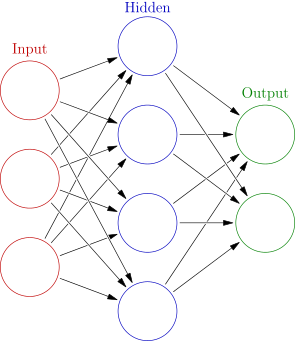
\includegraphics[scale=.5]{imatges/xnn.png}
	\caption{Xarxa neuronal}
\end{figure}
\subsection{Què és una neurona?}
\subsection{La funció d'activació}
\subsection{Com funcionen?}
\subsection{Com aprenen?}
\subsection{Descens del gradient}
\subsection{Descens del gradient estocàstic}
\subsection{Backpropagation}

\clearpage
\section{Classificació utilitzant una xarxa neuronal}
\subsection{Dades}
\subsection{Problema}
\subsection{Eines a utilitzar}
\subsection{Classificació}
Els passos a seguir per aplicar la classificació utilitzant una xarxa neuronal són.
\begin{enumerate}
	\item Preprocessament de les dades.
	\item Creació de la xarxa neuronal.
	\item Classificació.
	\item Evaluar la precissió del model.
\end{enumerate}
\subsubsection{Processament de les dades}

%%%%%%%%%%%%%%%BIBLIOGRAFIA%%%%%%%%%%%%%%%%%
\clearpage
\begin{thebibliography}{9}
	\bibitem{ANN}\textit{Xarxa neuronal}:
  	\\\path{https://en.wikipedia.org/wiki/Artificial_neural_network}
\end{thebibliography}

\clearpage
\begin{appendices}
\section{Codi}
\end{appendices}
\end{document}